\documentclass[a4paper,10pt]{article}
\usepackage[utf8]{inputenc}
\usepackage{amsmath}
\usepackage{graphicx}

\usepackage{hyperref}

%opening
\title{$^6$He CRES DAQ Design}
\author{Brent Graner}

\begin{document}

\maketitle

\begin{abstract}
This document outlines the organization of the data acqusition (DAQ) software for the $^6$He CRES experiment. Beginning from the design principles, consideration is given to the simplest means of overcoming the ambiguity introduced into Doppler-shifted signals, as well as the most efficient way to organize data processing without loss of frequency/energy resolution. The ROACH2 bitcode is introduced and discussed, along with installation tips for getting up to speed on development work.
\end{abstract}

\section{Doppler shift}
The axial motion of a radiating electron in a magnetic trap will cause the signal recieved by an on-axis observer to be modulated in frequency each time the electron reverses direction. The magnitude of the Doppler shift (proportional to the electron's maximum axial velocity) and the frequency of axial oscillation together define the $\textit{modulation index}$, denoted here as $h$:
\begin{equation}
 h = \frac{2\pi z_mf_c}{v_p}
\end{equation}
where $f_c$ is the cyclotron frequency, $z_m$ is the maximum axial displacement of the electron from the center of the trap, and $v_p$ is the (frequency-dependent) phase velocity of the waveguide mode of interest (in our case, the TE$_{10}$ mode).

The sidebands induced in a Doppler-shifted wavetrain at high modulation index make it difficult to unambiguously identify the cyclotron frequency. The effect of frequency modulation due to the axial motion of the trapped electron is illustrated in Figure \ref{red_wavetrain}. At a modulation index of 2.41, the carrier disappears and all received power is shifted into a large number of sidebands on either side. If the SNR is poor in the $^6$He data, fewer sidebands may stand out above the noise floor, making unambiguous identification of the carrier frequency nearly impossible. The modulation index may be suppressed by decreasing the trap depth, at the cost of a substantial decrease in the rate of detected events. To accept a non-negligible fraction of electrons, the trap must be deep enough to include particles with a modulation index greater than 2. 

\begin{figure}
\begin{center}
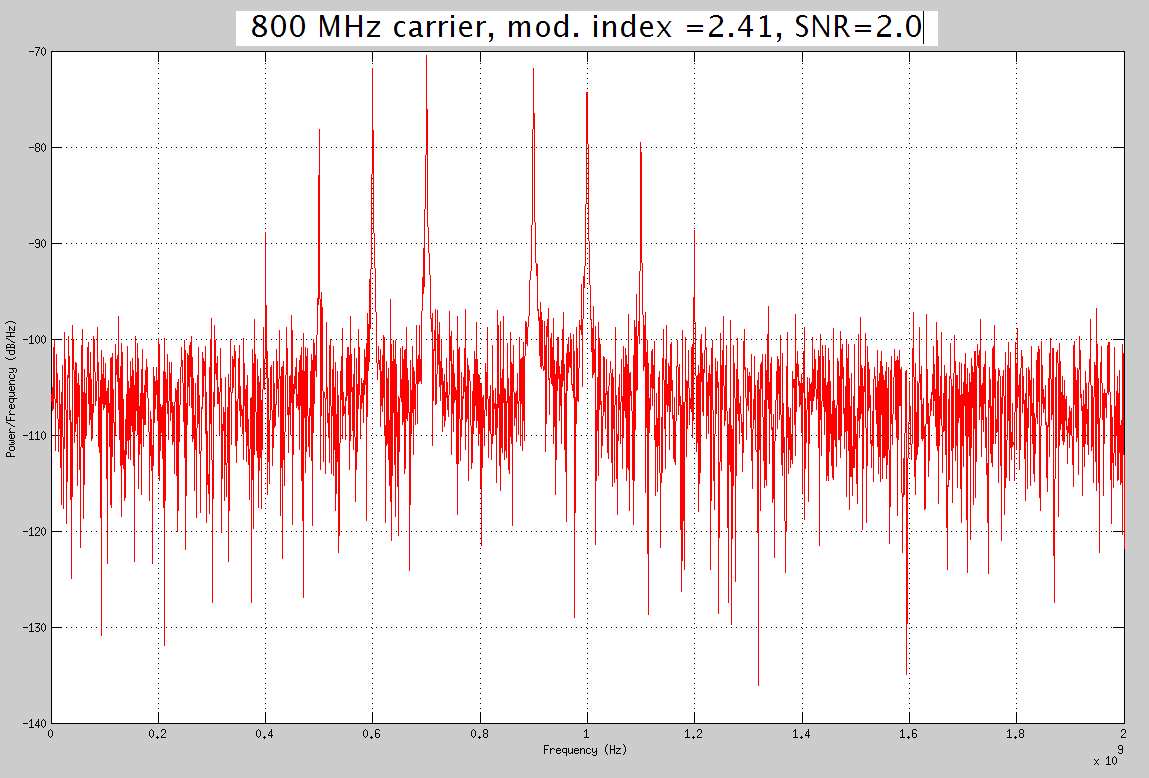
\includegraphics[scale=0.3]{Figures/800_MHz_red.png}
\end{center}
\caption[Red-shifted_PSD]%
{\narrower Plot of simulated power versus frequency for an 800 MHz electron with a signal/noise power ratio of 2.0, an axial trap oscillation frequency of 100 MHz, and a modulation index of 2.41.}
\label{red_wavetrain}
\end{figure}

\begin{figure}
\begin{center}
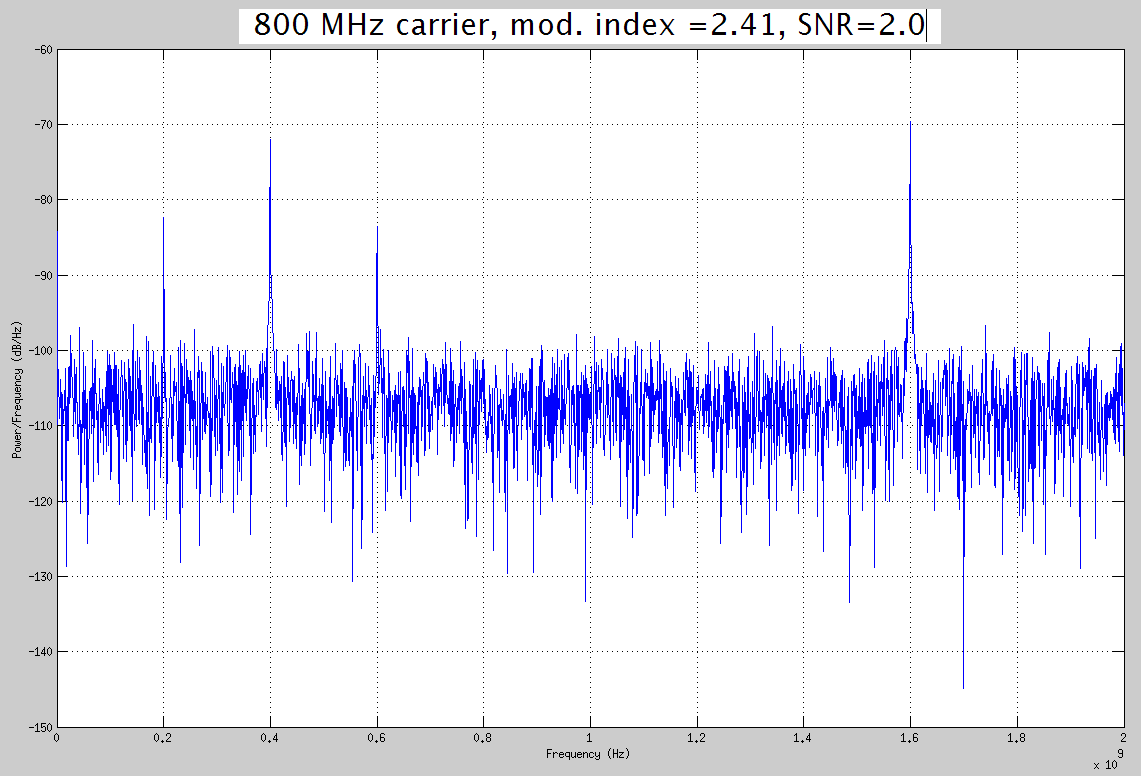
\includegraphics[scale=0.3]{Figures/800_MHz_prod.png}
\end{center}
\caption[Red-shifted_PSD]%
{\narrower Plot of simulated power versus frequency for the same 800 MHz electron with red-shifted and blue-shifted wavetrains multiplied together following digitazation with 2 8-bit 5Gs/sec ADC cards.}
\label{prod_wavetrain}
\end{figure}

Because a dual-receiver experiment is feasible, the simplest way to eliminate the Doppler shift as a source of uncertainty is to digitize the signals from both ends of the waveguide. Then one amplifier will output a red-shifted wave, while the other amplifier will output a blue-shifted one\footnote{There will be a path-length difference of order 10 cm between the decay volume and either end of the waveguides as they exit the magnet bore, but the low frequency of axial oscillation implies the red-shifted and blue-shifted wavetrains will be several meters long, so 2 amplifers situated at the same value of $z$ will almost always see waves with opposite Doppler shift. If necessary, the residual effect can be compensated by extending the waveguide arm without a 180-degree bend farther away in $z$ from the decay volume.}. The downmixed signals can be digitally multiplied and Fourier transformed, which will yield peaks at the sum and difference frequencies. The sum signal of the red-shifted and blue-shifted wave will be at twice the cyclotron frequency, giving an unambiguous way to identify the carrier from any set of sidebands.

The drawback to this method is the limitations imposed by the Nyquist theorem and a finite sampling rate. Instead of being limited to features less than half the frequency of the sampling, we will be limited to seeing cyclotron radiation at less than 1/4 of the ADC sampling frequency. In practice, this means that we will be able to see only cyclotron radiation less than 1.25 GHz above the frequency of the analog downmixing LO. Given that the ambiguity in the Doppler shifted waveforms is a considerable technical challenge, it seems that this is a viable tradeoff. We can put a bandpass filter on the analog RF output from 0.1 to 1.1 GHz, and the minimum cyclotron frequency can be placed in the baseband by tuning the value of the magnetic field $B_0$.

\section{Introduction to the CASPER and ROACH2 systems}
The DAQ system for the He6CRES experiment is based on a ROACH2\footnote{Reconfigurable Open Architecture Computing Hardware (version 2)} FPGA\footnote{Field Programmable Gate Array} system designed by the CASPER\footnote{Collaboration for Astronomical Signal Processing and Electronics Research} collaboration. The FPGA is programmed through a graphical interface (similar in style to National Instruments LabVIEW) that divides the FPGA chip into various `blocks' with dedicated input and output pins. However, information does not flow through the FPGA in the manner of a traditional processor, where the software is reducible to a list of operations to be executed sequentially on data that is accessed and stored in memory. In an ideal FPGA design, each block operates on each input and output pin on each clock cycle, as if all the functions in a typical software program were called simultaneously on a continuous stream of inputs. This design enables enormous throughput, but is complicated and unintuitive for a traditional programmer to conceptualize. 

The FPGA was provided to us from Xilinx, and is programmed using the Xilinx Simulink software package with ISE. The following sections give an explanation of the DAQ system, beginning with a description of the software stack necessary to program and compile bitcode. The remaining sections are devoted to explaining the  \texttt{he6\_cres\_correlator.slx} model file in further detail, as well as the low-level libraries available for interacting with the ROACH2 once it has been programmed.

\section{CASPER Library and Xilinx ISE Installation}
This section details the installation of the software needed to compile FPGA designs into bitcode that can be loaded directly onto the ROACH2 and is meant to help people through the inevitable compatibility issues encountered in the installation process. Readers who are not interested in installing the software to develop bitcode themselves should skip to the next section. 
\vspace{4mm}

I achieved a semi-stable configuration using the following list as described at
\href{https://casper.berkeley.edu/wiki/MSSGE\_Setup\_with\_Xilinx\_14.x\_and\_Matlab\_2012b}{https://casper.berkeley.edu/wiki/MSSGE\_Setup\_with\_Xilinx\_14.x\_and\_Matlab\_2012b}

\begin{enumerate}
\item Ubuntu 16.04
\item MATLAB R2012b + valid license file
\item Xilinx ISE version 14.7 system edition with System Generator
\item CASPER libraries mlib\_devel (switched to the ROACH2 branch)
\item A valid Xilinx license file
\item Linked versions of make and gmake
\end{enumerate}
\vspace{1mm} 

\hangindent=1.0cm 1) Ubuntu 16.04: This is what I took as a starting point. If you have total freedom, CASPER recommends Ubuntu version 12.04 or 14.04. Xilinx ISE 14.7 and MATLAB will work on Windows 7, but I don’t know how the CASPER libraries could be installed without /bash.
\vspace{3mm} 

\setlength{\parindent}{0.5cm}
\hangindent=1.0cm 2) MATLAB R2012b can be downloaded from the Mathworks website, although you will need to manually select and download a substantial number of packages. Per the instructions from Mathworks, just put all the .zip files in a directory, unzip the installer, execute it in a terminal, and go through the steps in the GUI.
\vspace{3mm} 

\setlength{\parindent}{1cm}\hangindent=1.0 cm pitfall: Mathworks licensing authentication servers require an internet connection configured as `eth0'. If your machine (like mine) has no physical ethernet jack, your wireless connection will be named something like `wlan0' by default.
\vspace{3mm}

\hangindent=1.0cm workaround: (as described at \href{https://askubuntu.com/questions/767786/changing-network-interfaces-name-ubuntu-16-04}{https://askubuntu.com/questions/767786 /changing-network-interfaces-name-ubuntu-16-04}):  run \texttt{ifconfig} to check whether or not your machine has an eth0 interface. If not, navigate to (or create) the directory eth/udev/rules.d and edit (or create) the file called 70-persistent-net.rules (you may also have to change the directory permissions using \texttt{chmod} or \texttt{chown}). Add the following line to 70-persistent-net.rules, replacing the 12 “X” characters with the digits of your machine’s MAC address:
\vspace{3mm} 

\hangindent=1.0cm SUBSYSTEM=="net", ACTION=="add", DRIVERS=="?*", ATTR{address}=="XX:XX:XX:XX:XX:XX", ATTR{dev\_id}=="0x0", ATTR{type}=="1", NAME="eth0"
\vspace{3mm} 

\hangindent=1.0cm Reboot and run \texttt{ifconfig} again to verify that your changes have taken effect.
\vspace{3mm} 

\setlength{\parindent}{0.5cm}
\hangindent=1.0cm 3) Xilinx ISE version 14.7 system edition with System Generator: Version 14.7 is the latest iteration that can be used to program the Xilinx Vertex 6, and by extension, the ROACH2. Packages can be downloaded from
\href{https://www.xilinx.com/support/download/index.html/content/xilinx/en/downloadNav/design-tools/v2012\_4---14\_7.html}{https://www.xilinx.com/support/download/index.html/content/xilinx/en /downloadNav/design-tools/v2012\_4---14\_7.html}
\vspace{3mm} 

\setlength{\parindent}{1cm}
\hangindent=1.0cm Instructions can be found at
\href{https://github.com/casper-astro/mlib\_devel/wiki/How-to-install-Xilinx-ISE}{https://github.com/casper-astro/mlib\_devel /wiki/How-to-install-Xilinx-ISE}
\vspace{3mm} 

\hangindent=1.0cm pitfall: Install the ``System'' edition, as opposed to the “WEB PACK” or “embedded” development kit. Be sure to edit the LD\_LIBRARY\_PATH variable in ALL THREE of the following .settings64.sh files:
\vspace{3mm} 

\hangindent=1.0cm Xilinx/14.7/ISE\_DS/common/.settings64.sh 

\hangindent=1.0cm Xilinx/14.7/ISE\_DS/EDK/.settings64.sh 

\hangindent=1.0cm Xilinx/14.7/ISE\_DS/ISE/.settings64.sh
\vspace{3mm} 

\hangindent=1.0cm If you don’t have all three of the above directories, you need to change the edition of ISE design suite you installed.
\vspace{3mm} 

\setlength{\parindent}{0.5cm}
\hangindent=1.0cm 4) CASPER libraries mlib\_devel (switched to the ROACH2 branch): Clone the ROACH2 branch of the libraries by running \texttt{git clone -b roach2 https://github.com/casper-astro/mlib\_devel/tree/roach2}
\vspace{3mm} 

\hangindent=1.0cm 5) License file: Xilinx donates licenses through it's university program; it takes a few days to be approved and each license is `node-locked' so that it can be run on one and only one machine. If you don't want to do the paperwork or wait, I have some extra licenses--ask and ye shall receive. Whoever you get it from, run the License Configuration Manager \texttt{xlcm} and navigate to the folder where you keep your license file to install it. 
\vspace{3mm} 

\hangindent=1.0cm 6) Another potential pitfall at compile time involves the use of gmake. Ubuntu has both make and gmake  installed by default, but they may need to be linked. Use the command \texttt{sudo ln -s /usr/bin/make /usr/bin/gmake} to create a symbolic link to gmake.

\section{Input signal digitization}
The current design of the \texttt{he6\_cres\_correlator} includes 2 ADC1x5000-8 (aka ASIAA 5Gsps ADC) cards. Our models use the DMUX 1:1 multiplexing configuration (set in hardware), which outputs two 8-bit samples per ADC clock cycle\footnote{The other available option is DMUX 1:2, which outputs four 4-bit streams per ADC clock cycle}. The ADC is run off an external clock input with a maximum rate of 2.5GHz, which equates to 5 GS/sec. However, Andre Young has advised us that the ADC response becomes distorted at the highest possible frequencies, so the target sampling rate is set to 4 GHz (or a 2000 MHz ADC clock). The corresponding CASPER software `yellow block' features 16 parallel outputs, two of which are filled on each ADC clock cycle. The FPGA should therefore be clocked at 1/8 times the rate of the ADC clock.

The ADC can be also be operated in dual-channel mode, putting two different analog signals into a single ADC card, with one sample per SMA channel per ADC clock cycle. In single-channel mode, one SMA input is connected, and the ADC card gives 2 samples per clock cycle. We will use the single channel mode, so the clock frequency will be half that of the sampling frequency (cf. https://www.mail-archive.com/casper@lists.berkeley.edu/msg06356.html) 

The ADC has an analog input range of $\pm$250 mV, and the values output from the yellow asiaa\_adc5g yellow blocks are encoded as fixed point two's complement numbers with 8.7-bits each, meaning that the most sigificant bit (MSB) inidicates the sign, while the 'binary point' is understood to come between the MSB and the 7 LSB. This gives $2^8=256$ possible representaions of the normalized input. For further explanation of the nomenclature, see \href{https://casper.berkeley.edu/wiki/Wideband\_Spectrometer}{https://casper.berkeley.edu/wiki/Wideband\_Spectrometer}

\section{Fixed-point multiplication}
ADC outputs are sent to the multipliers subsystem, where each simultaneous pair of voltage samples is multiplied. Because there are 7 bits representing the magnitude of the ADC voltage sample, there will be $2^7 \cdot 2^7$ possible magnitudes for the product. Including the sign bit, the products can be stored as 15.14 bit fixed-point values without any loss of resolution. 

\section{Polyphase filter bank}
The output of the Multiplier section is entered into a polyphase filter bank block which applies Finite Imulse REsponse (FIR) digital filters to reduce flaws in the discrete Fourier transform algorithms including spectral leakage, etc. The filters are implemented by digitally multiplying input data points with sinc function windows. This is an extrememly important topic and is treated extensively in the book by Smith, which may be downloaded free of charge at \texttt{http://www.dspguide.com/}. The input bitwidth is set to 15 bits to match the multiplier output. The PFB will take $2^{14}$ time samples as input, which will be the same as the input fed to the FFT.

\section{Fourier transform}
The FFT algorithm of choice is a 12-stage butterfly biplex Fourier transform. Note that the FFT takes $2^{14}$ real values as inputs and gives $2^{13}$ complex values as output. One thing to note about the CASPER designs is the apparent convention for representing complex numbers as fixed-point quantities. Many of the CASPER blocks incoporate a \texttt{BitWidth} setting, and operate using ``A complex number whose higher BitWidth bits are its real part and lower BitWidth bits are its imaginary part''. This is only relevant to the FFT block because it's the only block in the program that takes real (time-domain) samples as input, and returns complex (frequency domain) points as output. The real and imaginary pats of a given fequency bin are output simultaneously on each clock cycle for a given 'pin'. This explains why the number of output 'pins' is half the number of inputs).

Since we are interested in a specrogram of power vs. frequency, it is more appropriate to work with the mod squared of each FFT channel. Each power block slices each complex output into two 18.17-bit samples (in two's complement binary representation), then squares both real and imaginary parts and adds them. The output of the adder blocks is rounded to 8 bits, so with a 250 MHz FPGA clock and 64 bits of output on each clock cycle, we anticipate 2000 MB/sec of output. The mod squared values of the FFT are non-negative by definition, so we can get the best resolution out of 8 bits by dropping the two's complement representation convention at this point and treating the outputs as unsigned binary numbers.

\section{Packetization}
The simplest and most direct way to packetize the data would be to output one power spectrum per packet. The typical packets used by Project 8 have a payload of 8192 bytes each. To see if it is feasible to write a full spectrum in one such packet, we must consider the resolution attainable in writing a 2 GHz frequency region of interest (noting that we are interested in the sum frequency of two inputs each $\leq$ 1 GHz to remove the Doppler shift and still be below half the ADC sampling frequency). With 1 byte output for each of the 8192 frequency channels of the FFT, we can fit 8192 frequency channels per packet. Assuming the typical cyclotron frequency is approximately 19 GHz, the frequency resolution is 
\begin{equation}
\frac{2 \text{ GHz}}{19 \text{ GHz}}*\frac{1}{8192} =   1.28*10^{-5}
\end{equation}
or about 12 ppm resolution of the average cyclotron frequency, well within acceptable limits. 

The other dimension of resolution to consider is the time slice parameter on a waterfall plot. With $2^{14}$ points in each FFT and a sampling frequency of 4 GHz, each power spectrum will take $4.1 \mu\text{s}$ to capture. This is about a factor of 7 shorter than the time resolution of the Project 8 plots, which are $30 \mu \text{s}$ long.

The packetization block (and the overall packet structure) are lifted from the Project 8 design alternately known as r2daq or ArtooDaq. We retain the 8192-byte payload and 64-byte header, which includes metadata such as timestamps, packet number, analog channel, and some extra space reserved for future use.

\section{Power spectrum output}
The ROACH2 module has a single breakout card with 4 x 10 Gb/sec Ethernet ports. The output data rate of 2000 MB/sec (or $\approx$16 Gb/sec) will therfore require us to use multiple ports. The output of each successive packet is toggled between the four 10GbE SFP+ ports, designated tengbe\_a, tengbe\_b, and so on. 

\section{Phasmid library and installation tips}
The Project 8 software module called phasmid is located at \href{https://github.com/project8/phasmid}{https://github .com/project8/phasmid}. This module contains the lowest-level library r2daq.py for interacting with the ROACH2, programming the FPGA with some pre-compiled bitcode, getting and setting values from the software registers, as well as calibrating offset, gain, and phas parameters of individual ADC cores. A similar version, He6DAQ.py, is unique to the He6CRES ROACH2 setup and is currently being developed. 

To install phasmid:
\vspace{3mm}

1) Run \texttt{git clone https://github.com/project8/phasmid} 
\vspace{3mm}

2) Run \texttt{git clone https://github.com/sma-wideband/adc\_tests}
\vspace{3mm}

\hangindent=0.5cm
3) Change into directory containing lowest-level-ROACH2 interface library (r2daq.py or He6DAQ.py)
\vspace{3mm}

\hangindent=0.5cm
4) Copy adc\_5g folder from adc\_tests into same directory as r2daq.py or He6DAQ.py
\vspace{3mm}

5) Run \texttt{sudo pip install corr==0.7.3}
\vspace{3mm}

6) If scipy is not already installed, run \texttt{sudo pip install scipy}
\vspace{3mm}

7) If netifaces is not already installed, run \texttt{sudo pip install netifaces}
\vspace{3mm}

8) Run \texttt{sudo pip install construct==2.5.5-reupload}
\vspace{3mm}

If the installation is successful, you should be able to navigate to the folder with the DAQ library, boot up an interactive python session (run \texttt{ipython}), and run \texttt{import r2daq} or \texttt{import He6DAQ} without any error messages.

\section{Appendix: Throttling the output data rate}
If we find that 2000 MB/sec of output is unmanageable, we could theoretically limit the amount of data to be stored and copied by implementing an FFT averaging window. Instead of taking each FFT calculated by the FPGA and writing it to disk immediately, we could use buffers in the FPGA memory to average many of FFTs to output one packet with an expected SNR which improves as the square root of the number of samples to be averaged. 

While this tactic is not currently in the initial version of the ROACH2 bitcode, it would be limited by the change in cyclotron frequency as the electron loses energy--eventually the signal will migrate into the neighboring frequency bins\footnote{This estimate ignores the effect of relatively rare scattering events observed by Project 8, which cause the signal to abruptly `jump' up or down by several MHz.}. A 2 MeV electron has about $3\cdot10^{-13}$ J of kinetic energy. If we assume energy is lost at about $3\cdot10^{-15}$ W, the change in energy is about 1\% per second. Keeping the 10 ppm frequency resolution, we may ask how long it will take for an electron's frequency to migrate into the next bin. $10^{-4}$ s is equivalent to a frequency change of 1 ppm, so the output period for a packet should be at most 0.5 ms, or the expectation time for a random-frequency signal to move between frequency bins. This is easily-attainable, setting a floor on the output data rate of 8.2 KB/packet * 2000 packets/sec = 16.4 MB/s. This is nearly three orders of magnitude less than the 5 GB/sec necessary to contain raw time-domain data of 1 byte/sample taken at 5 GHz. 

In practice, however, we will want to have many FFTs with an electron in the same or adjacent frequency bins. Anecdotal evidence suggests Project 8 observes scattering events with an averge frequency of about 1 kHz, so we will want to output more than 2 FFTs per millisecond. We can easily leave this as an adjustable parameter in the code to balance competing needs for extended tracks on our waterfall plots on the one hand and manageable data rates on the other. 
\end{document}
